\documentclass{article}
\usepackage{graphicx}
\usepackage{courier}
\usepackage{listings}
\usepackage{color}

\definecolor{dkgreen}{rgb}{0,0.6,0}
\definecolor{gray}{rgb}{0.5,0.5,0.5}
\definecolor{mauve}{rgb}{0.58,0,0.82}

\lstset{frame=tb,
  language=Java,
  aboveskip=3mm,
  belowskip=3mm,
  showstringspaces=false,
  columns=flexible,
  basicstyle={\small\ttfamily},
  numbers=none,
  numberstyle=\tiny\color{gray},
  keywordstyle=\color{blue},
  commentstyle=\color{dkgreen},
  stringstyle=\color{mauve},
  breaklines=true,
  breakatwhitespace=true,
  tabsize=3
}


\begin{document}

\title{A Title}


\maketitle

\begin{abstract}
  Current Research of GUI testing focus on event sequences.
  They can't cover code.
  We can.
\end{abstract}

\section{Introduction}\label{section:introduction}
this is a place holder sentense.

\section{Example}

\begin{figure}
  \centering
  \caption{ticket example}
  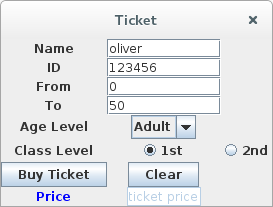
\includegraphics{./res/ticket.png}
\end{figure}

To demostrate  the importance of branch coverage testing of GUI applications, we will use a  \texttt{Ticket Seller} example application. Note that we borrowed the example from barad. Figure 1 shows the GUI of this \texttt{Ticket Seller} application.

This program is used to calculate ticket price according to different properties of the client, such as the class level, or age, or the travel distance. When the \texttt{Buy} button is clicked, the application check the \texttt{Name} and \texttt{ID} input, if the length of the \texttt{Name} string is less or equal than 3, or \texttt{ID} equals to some special string, then the application will display an error message and will not calculate any price. After checking the user information successfully, the application start to calculate the price as follows: read the user class input and set a coeffient for the price, read the user age to go to different pricing branch, read the start and dest input and calculate the distance of travelling, then calculate the price. We can see from the following code snippets that there should be many branches in the code to calculate ticket price for all kinds of clients.

\begin{lstlisting}
  int coeficient = (classLevel == TicketModel.FIRSTCLASS) ? 1 : 2;
  int dist = to - from;
  if (ageLevel == 1) {
    if (dist < 40) {
      price = 100 * coeficient;
    } else if (dist < 45) {
      price = 110 * coeficient;
    } else if (dist < 50) {
      price = 120 * coeficient;
    } else if (dist < 70) {
      price = 140 * coeficient;
    } else if (dist < 80) {
      price = 150 * coeficient;
    } else if (dist < 85) {
      price = 155 * coeficient;
    } else if (dist < 100) {
      price = 160 * coeficient;
    }
  }
\end{lstlisting}

One can not claim this kind of applications are well tested until all the branches has been covered during test stage.


\section{Inplementation}


\section{Related Work}\label{section:relatedwork}

\bibliographystyle{abbrv}
\bibliography{references}

\end{document}
